\section{Experimental details on CIFAR10}
\label{sec:app_cifar10}


In this section, we give the experimental details on the CIFAR10-based experiments shown in Figures \ref{fig:teaserplot} and \ref{fig:K_plot}. Moreover, we also conduct similar experiments using different neural network architectures. First, we give the full experimental details and then provide the results of the experiments using the different architectures.

\paragraph{Subsampling CIFAR10}
%CIFAR10 is an image dataset consisting of $50k$ training images of $10$ classes and $10k$ test images, where each class has a total of $6k$ images. 
In all our experiments we subsample CIFAR10 to simulate the low sample size regime. We ensure that for all subsampled versions the number of samples of each class are equal. Hence, if we subsample to $500$ training images, then each class has exactly $50$ images, which are drawn uniformly from the $5k$ training images of the respective class.

\paragraph{Mask perturbation on CIFAR10}
We consider square black-mask perturbations; the attacker can set in the image a patch of size $2 \times 2$ to zero. The attack is a simplification of the patch-attack as considered in \cite{Wu20}. We show an example of a black-mask attack on each of the classes in CIFAR10 in Figure \ref{fig:cifar10_masks}. Clearly, the mask reduces the information about the class in the image as it occludes part of the object in the image.

\begin{figure}[!ht]
\centering
  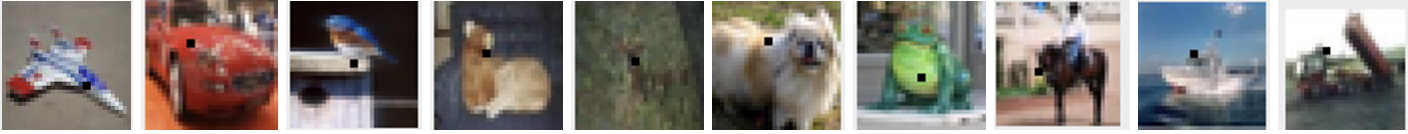
\includegraphics[width=0.8\linewidth]{plotsAistats/cifar10_black_mask_attack.png}
  \caption{We show an example of a mask perturbation for all $10$ classes of CIFAR10. Even though the attack occludes part of the images, a human can still easily classify all images correctly.}
\label{fig:cifar10_masks}
\end{figure}

During test time, we evaluate the attack exactly by means of a full grid search over all possible windows. Note that a full grid search requires $900$ forward passes to evaluate one image, which computationally too expensive during training time. Therefore, we use the same approximation as in \cite{Wu20} at training time. For each image in the training batch, we compute the gradient from the loss with respect to the input. Using that gradient, which is a tensor in $\mathbb{R}^{3 \times 32 \times 32}$, we compute the $l_1$-norm of each patch by a full grid search and save the upper left coordinates of the $K$ windows with largest $l_1$-norm. The intuition is that windows with high $l_1$-norm are more likely to change the prediction. Out of the $K$ identified candidate windows, we take the most loss worsening by means of a full list-search. 

\begin{wrapfigure}{r}{0.4\textwidth}
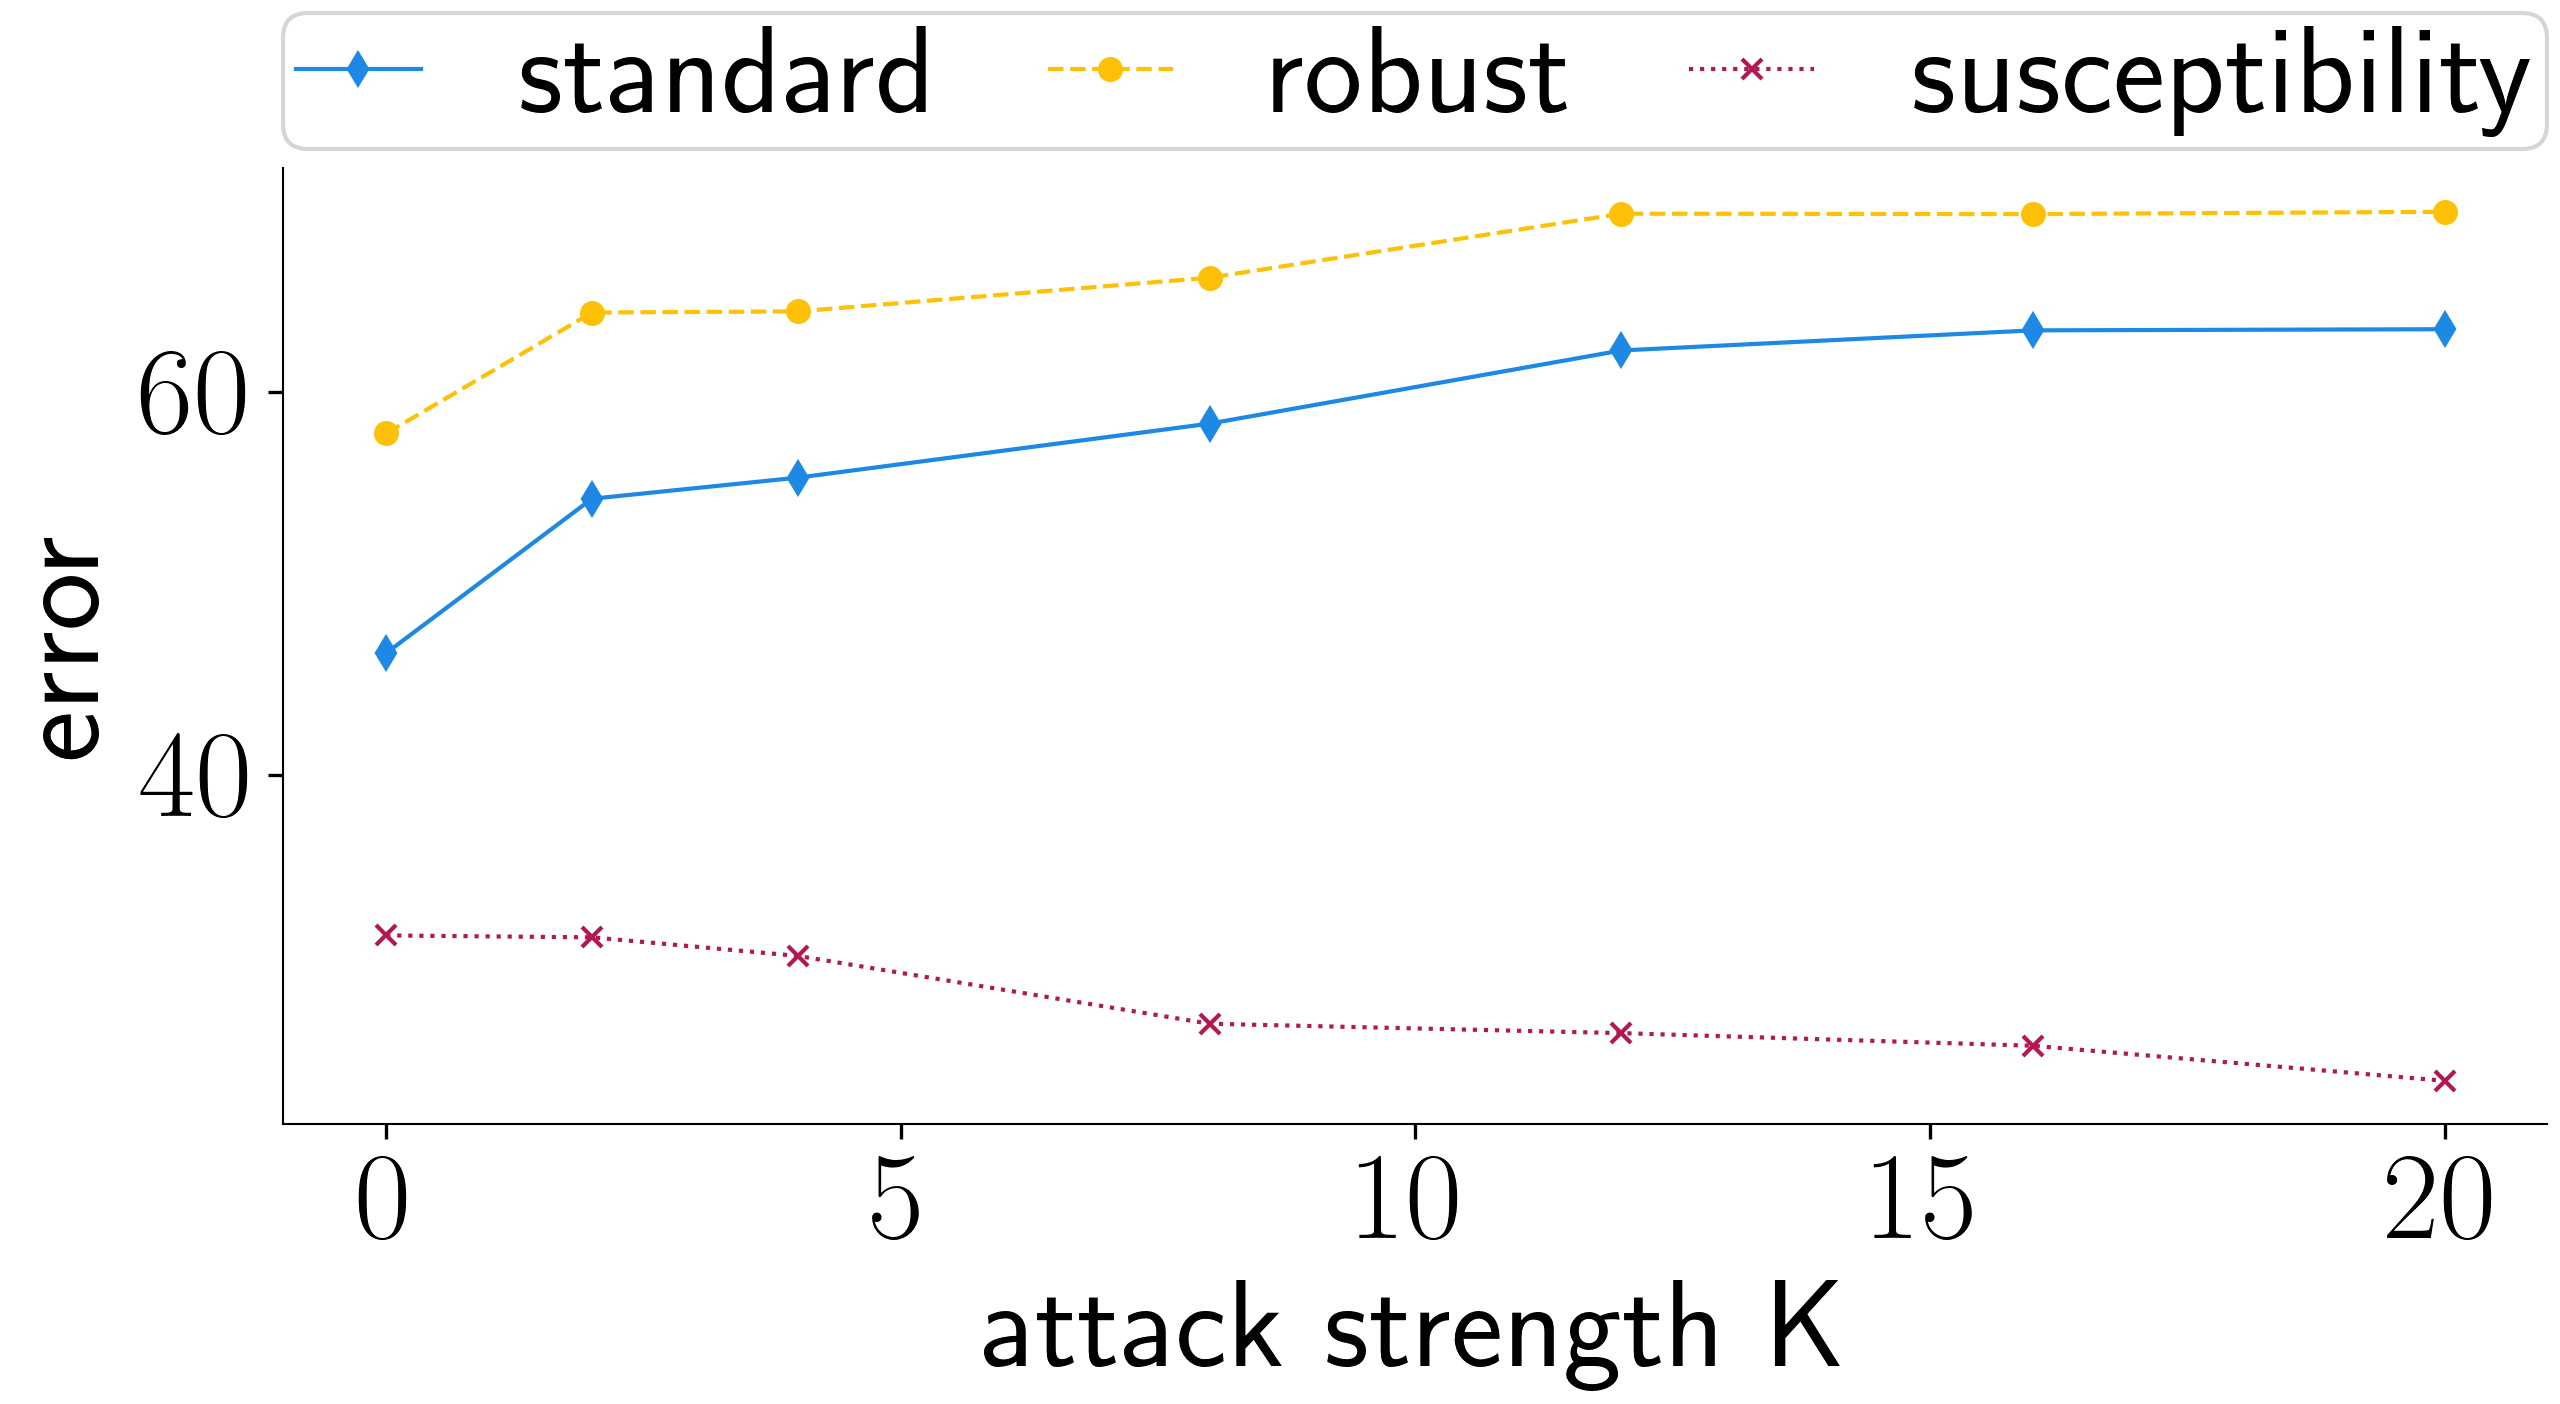
\includegraphics[width=0.99\linewidth]{plotsAistats/K_plot_cifar.png}
\caption{We plot the standard error, robust error and susceptibility for varying attack strengths $K$. We see that the larger $K$, the lower the susceptibility, but the higher the standard error.}
\label{fig:K_plot}
\end{wrapfigure}

\paragraph{Experimental training details}
For all our experiments on CIFAR10, we adjusted the code provided by \cite{Phan21}. As typically done for CIFAR10, we augment the data with random cropping and horizontal flipping. For the experiments with results depicted in Figures \ref{fig:teaserplot} and \ref{fig:K_plot}, we use a ResNet18 network and train for $100$ epochs. We tune the parameters learning rate and weight decay for low robust error. For standard standard training, we use a learning rate of $0.01$ with equal weight decay. For adversarial training, we use a learning rate of $0.015$ and a weight decay of $10^{-4}$. We run each experiment three times for every dataset with different initialization seeds, and plot the average and standard deviation over the runs. 

For the experiments in Figure \ref{fig:teaserplot} and \ref{fig:num_obs_CIFAR} we use an attack strength of $K = 4$. Recall that we perform a full grid search at test time and hence have a good approximation of the robust accuracy and susceptibility score. 

\paragraph{Increasing training attack strength} We investigate the influence of the attack strength $K$ on the robust error for adversarial training. We take $\epstrain = 2$ and $\numsamp = 500$ and vary $K$. The results are depicted in Figure \ref{fig:K_plot}. We see that for increasing $K$, the susceptibility decreases, but the standard error increases more severely, resulting in an increasing robust error. 


\paragraph{Robust error decomposition}
In Figure \ref{fig:teaserplot}, we see that the robust error increases for adversarial training compared to standard training in the low sample size regime, but the opposite holds when enough samples are available. For completeness, we provide a full decomposition of the robust error in standard error and susceptibility for standard and adversarial training. We plot the decomposition in Figure \ref{fig:num_obs_CIFAR}.

\begin{figure*}[!b]
\centering
\begin{subfigure}[b]{0.32\textwidth}
  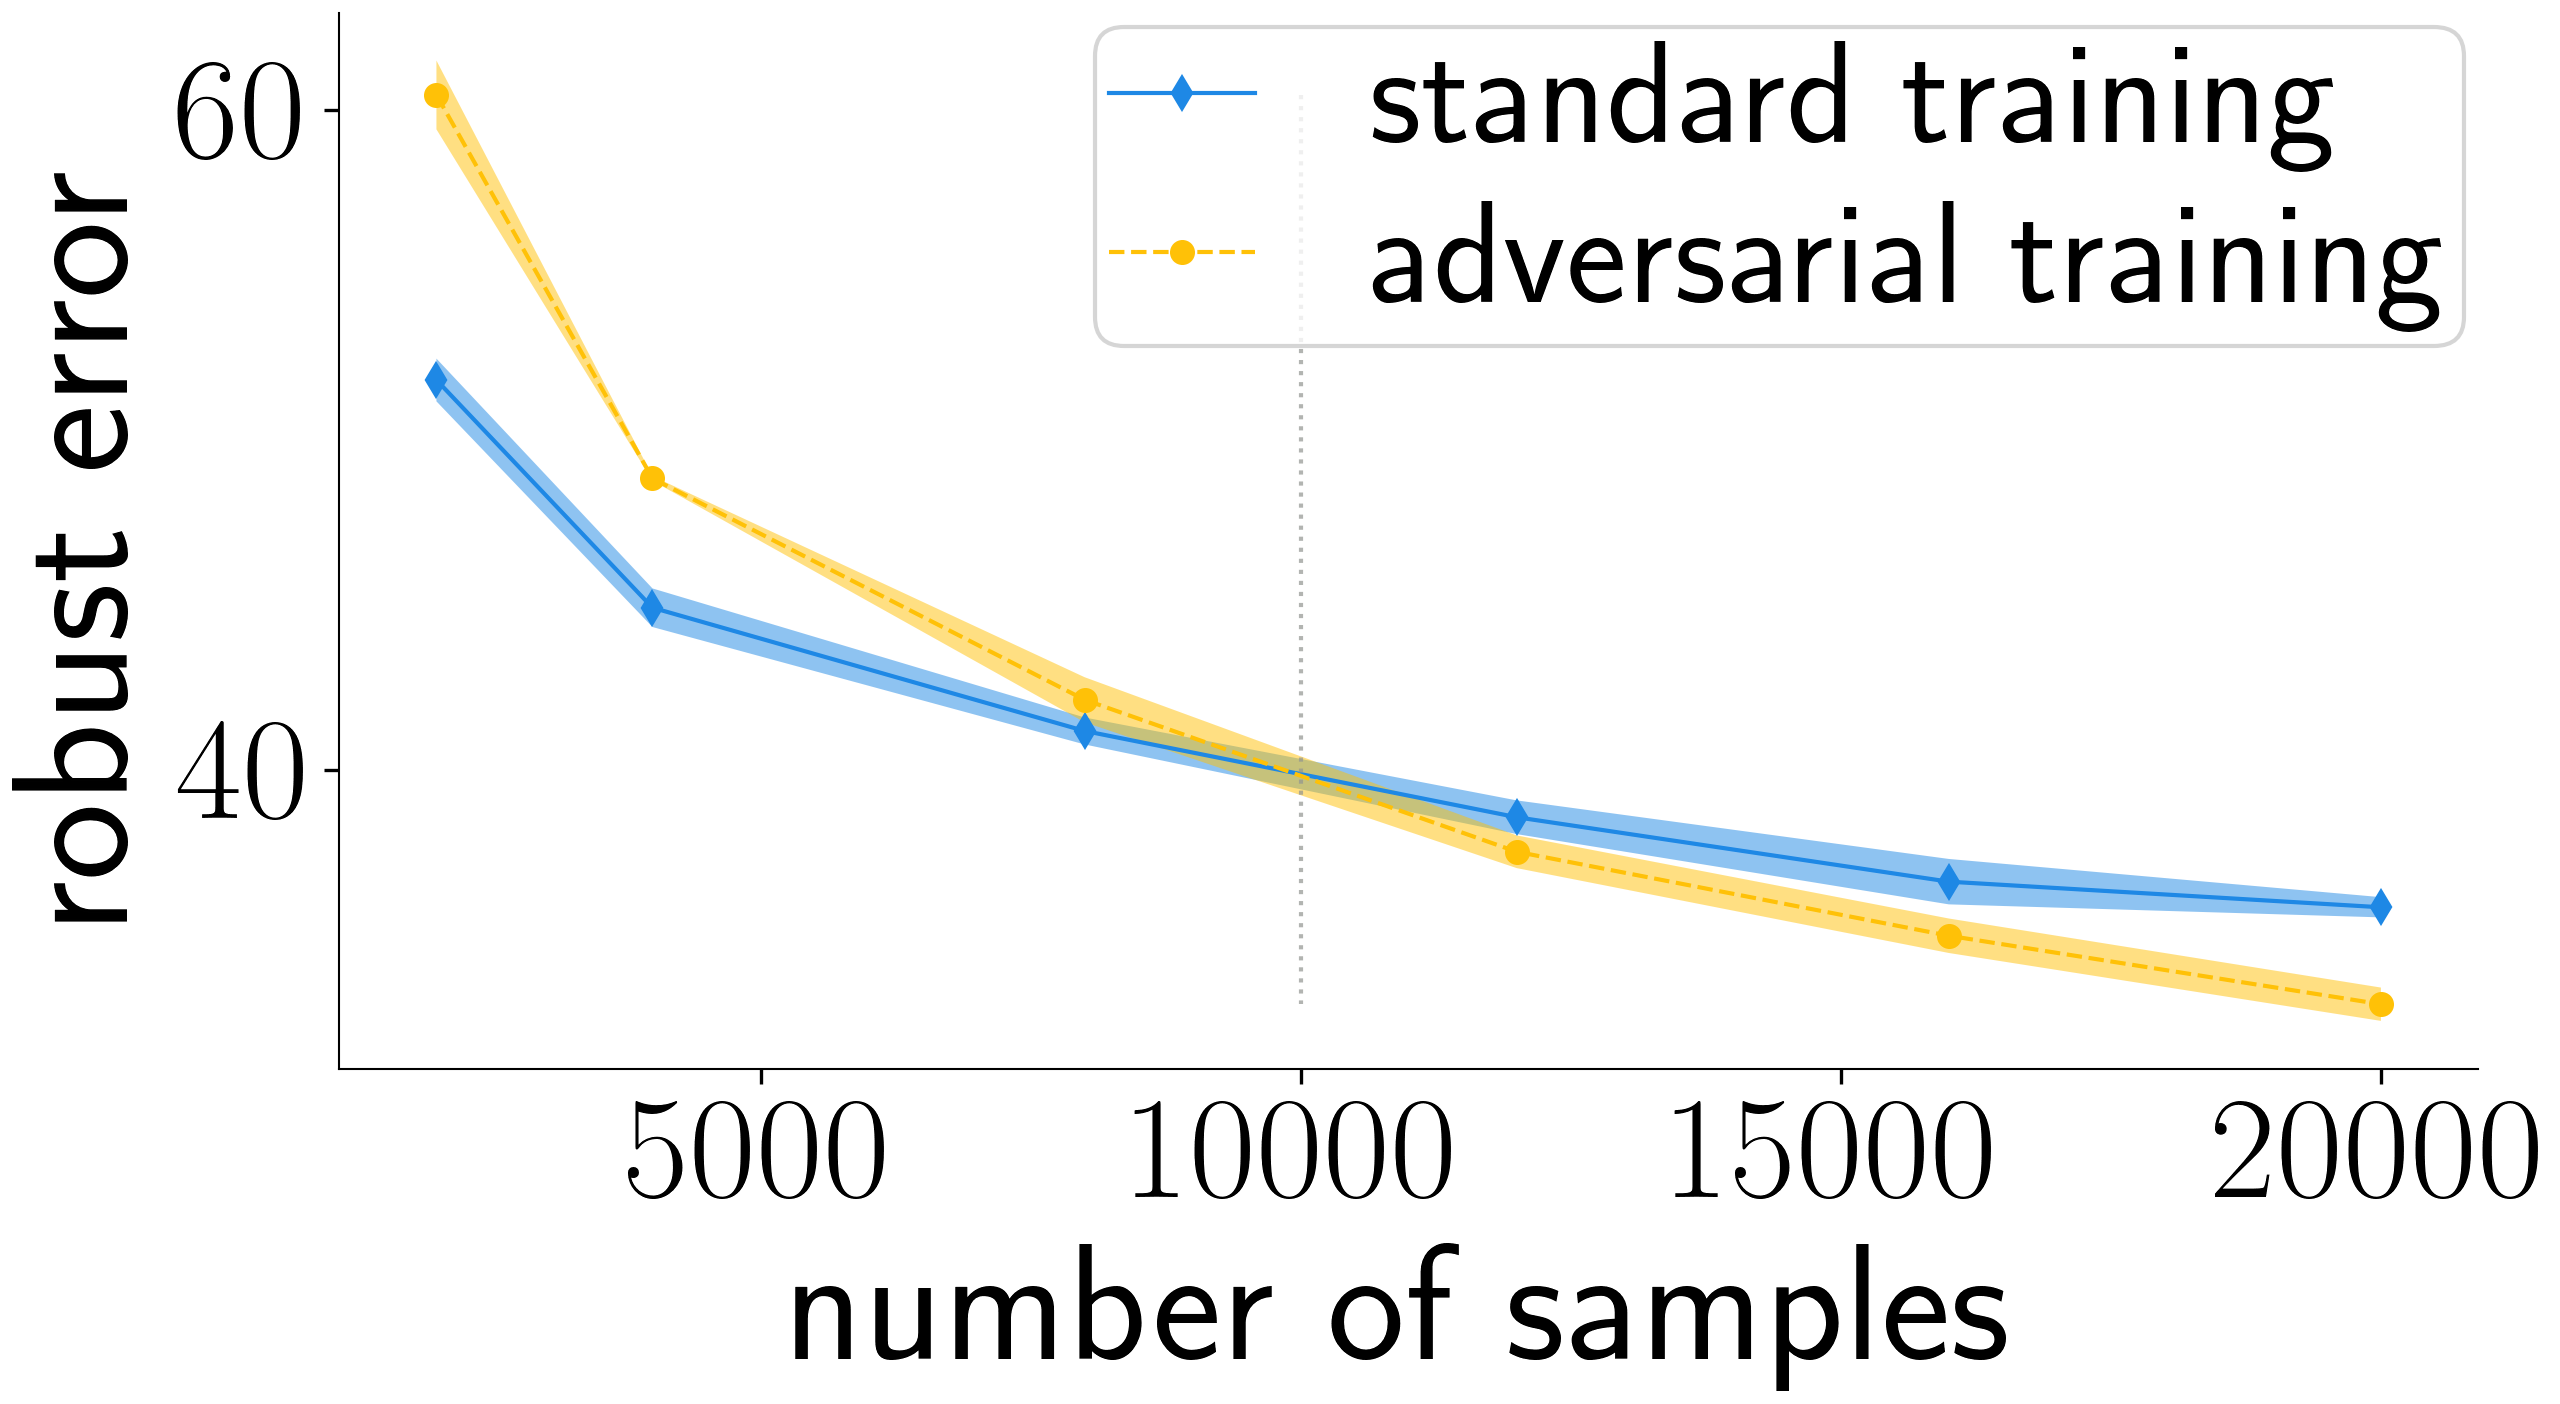
\includegraphics[width=0.99\linewidth]{plotsAistats/cifar10_robust_numobs.png}
  \caption{Robust error}
  \label{fig:RA_CIFAR_10_n}
\end{subfigure}
\begin{subfigure}[b]{0.32\textwidth}
  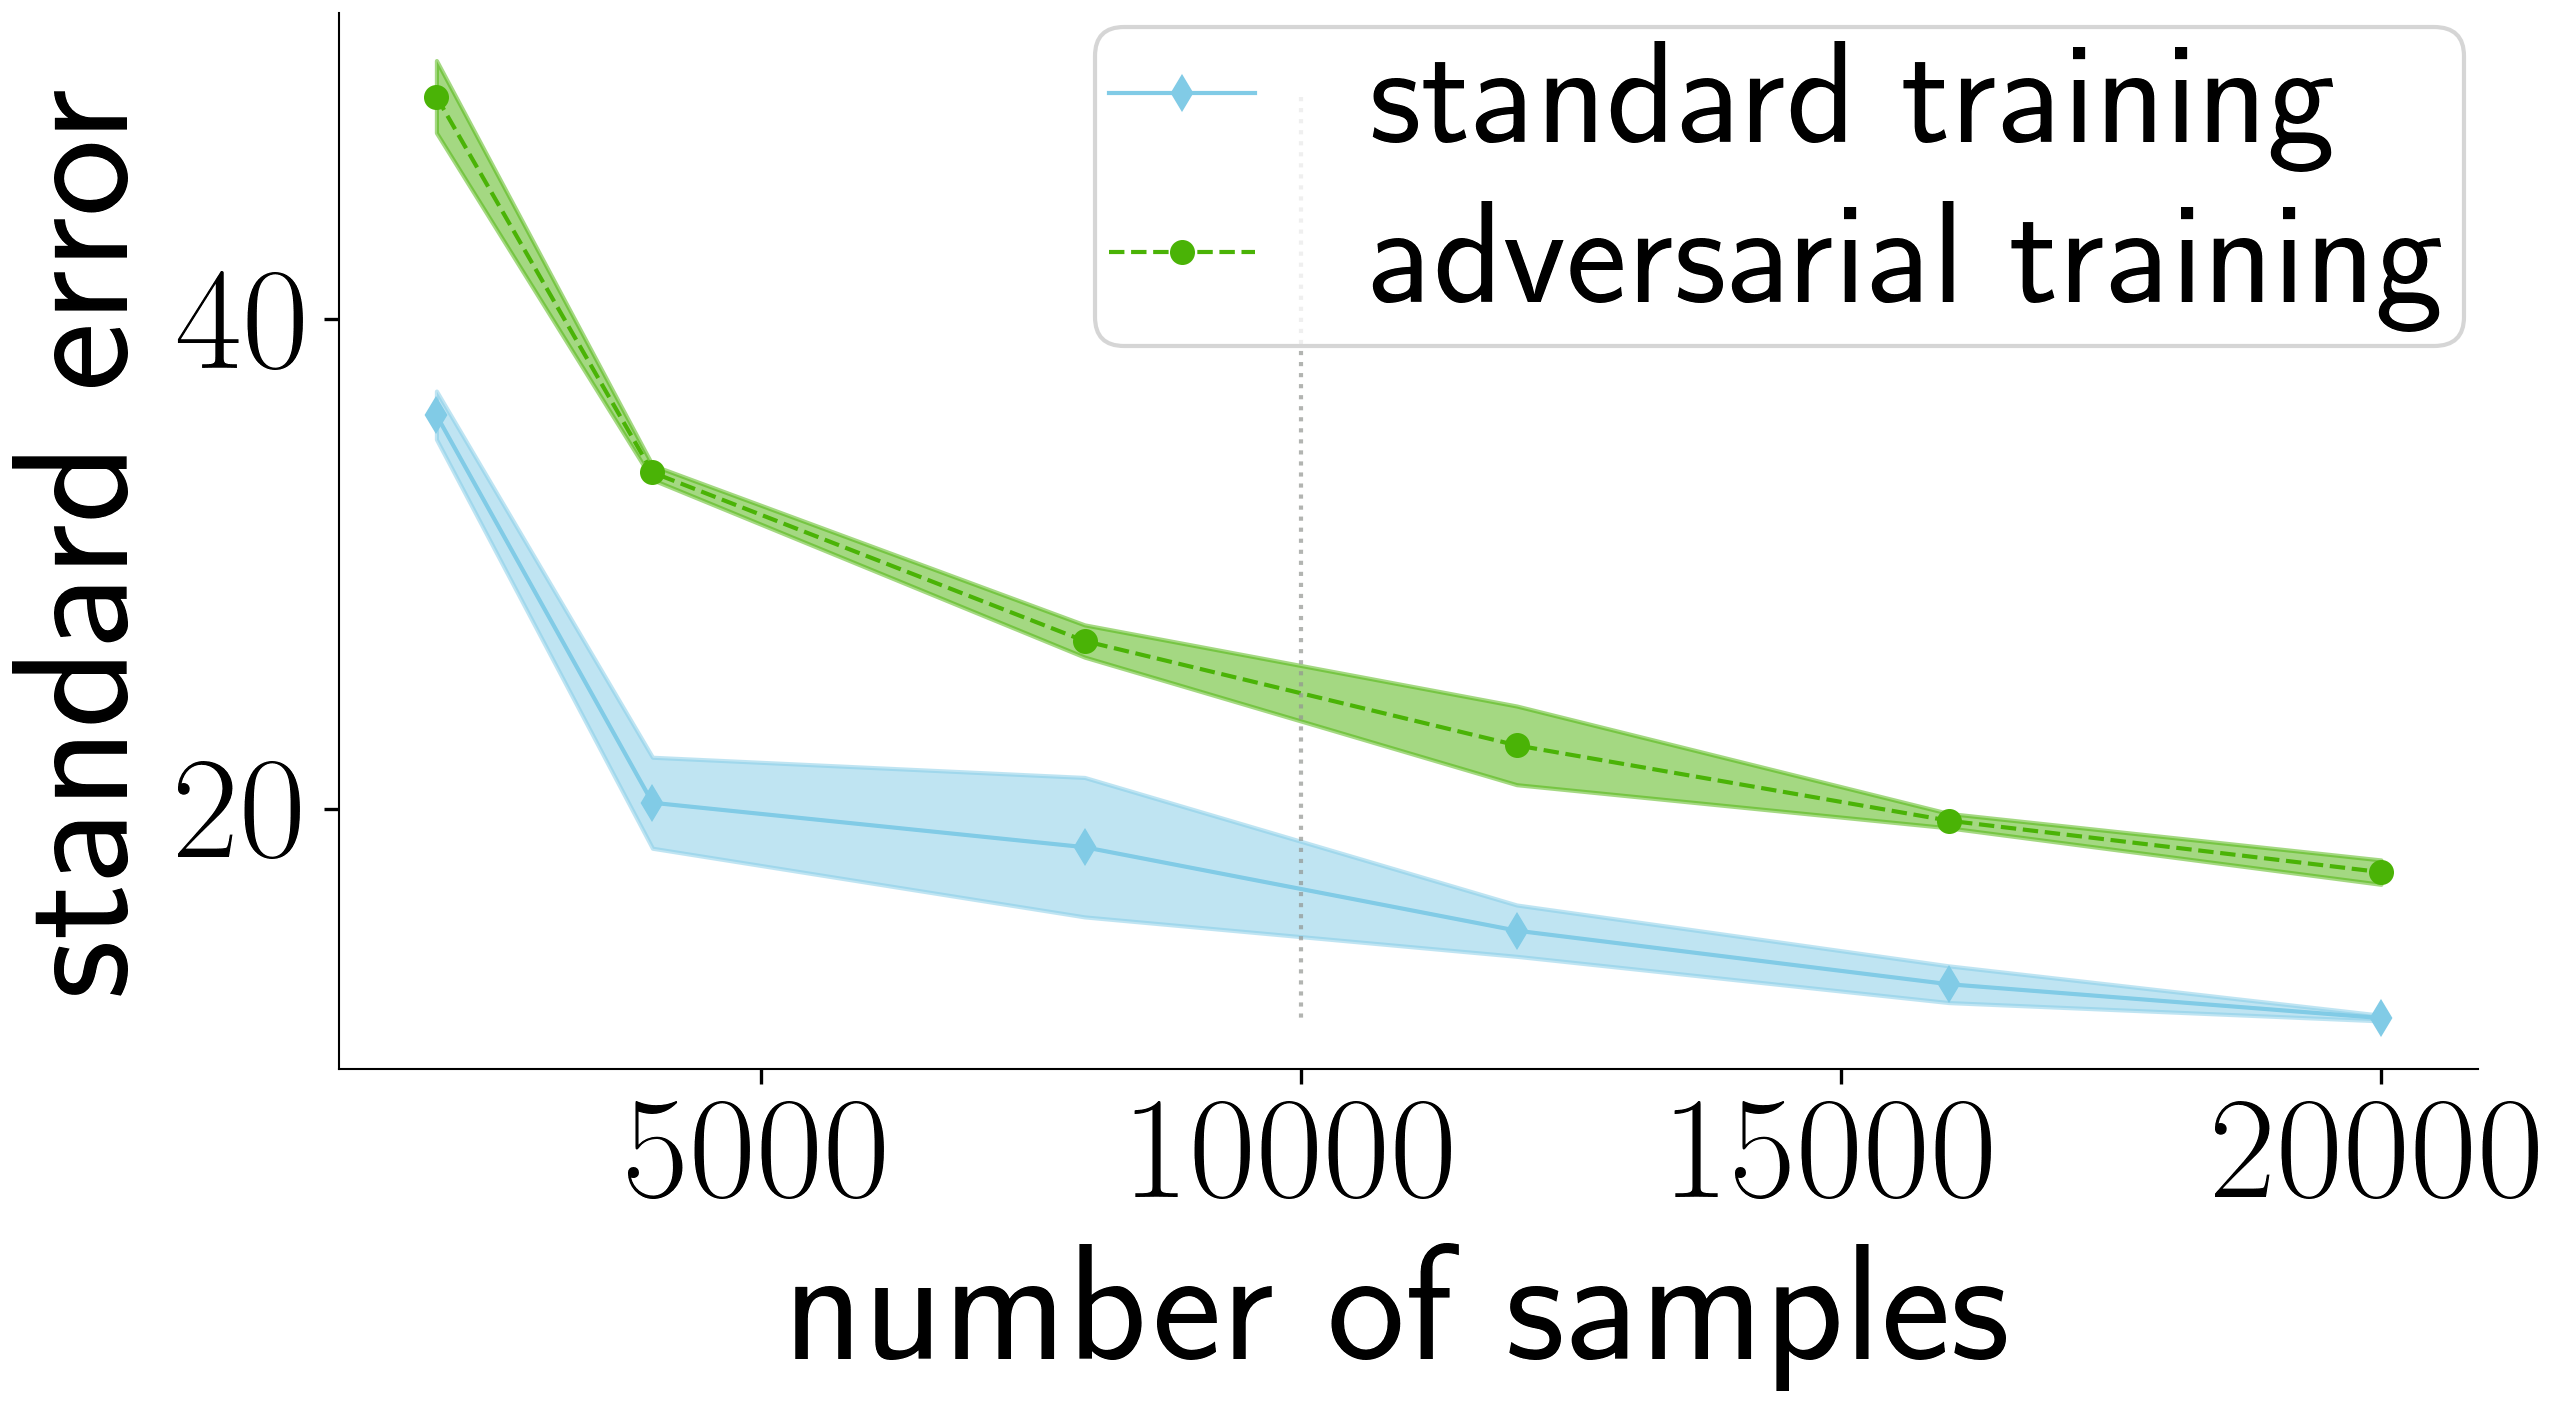
\includegraphics[width=0.99\linewidth]{plotsAistats/cifar10_standard_numobs.png}
  \caption{Standard error}
  \label{fig:SA_CIFAR_10_n}
\end{subfigure}
\begin{subfigure}[b]{0.32\textwidth}
  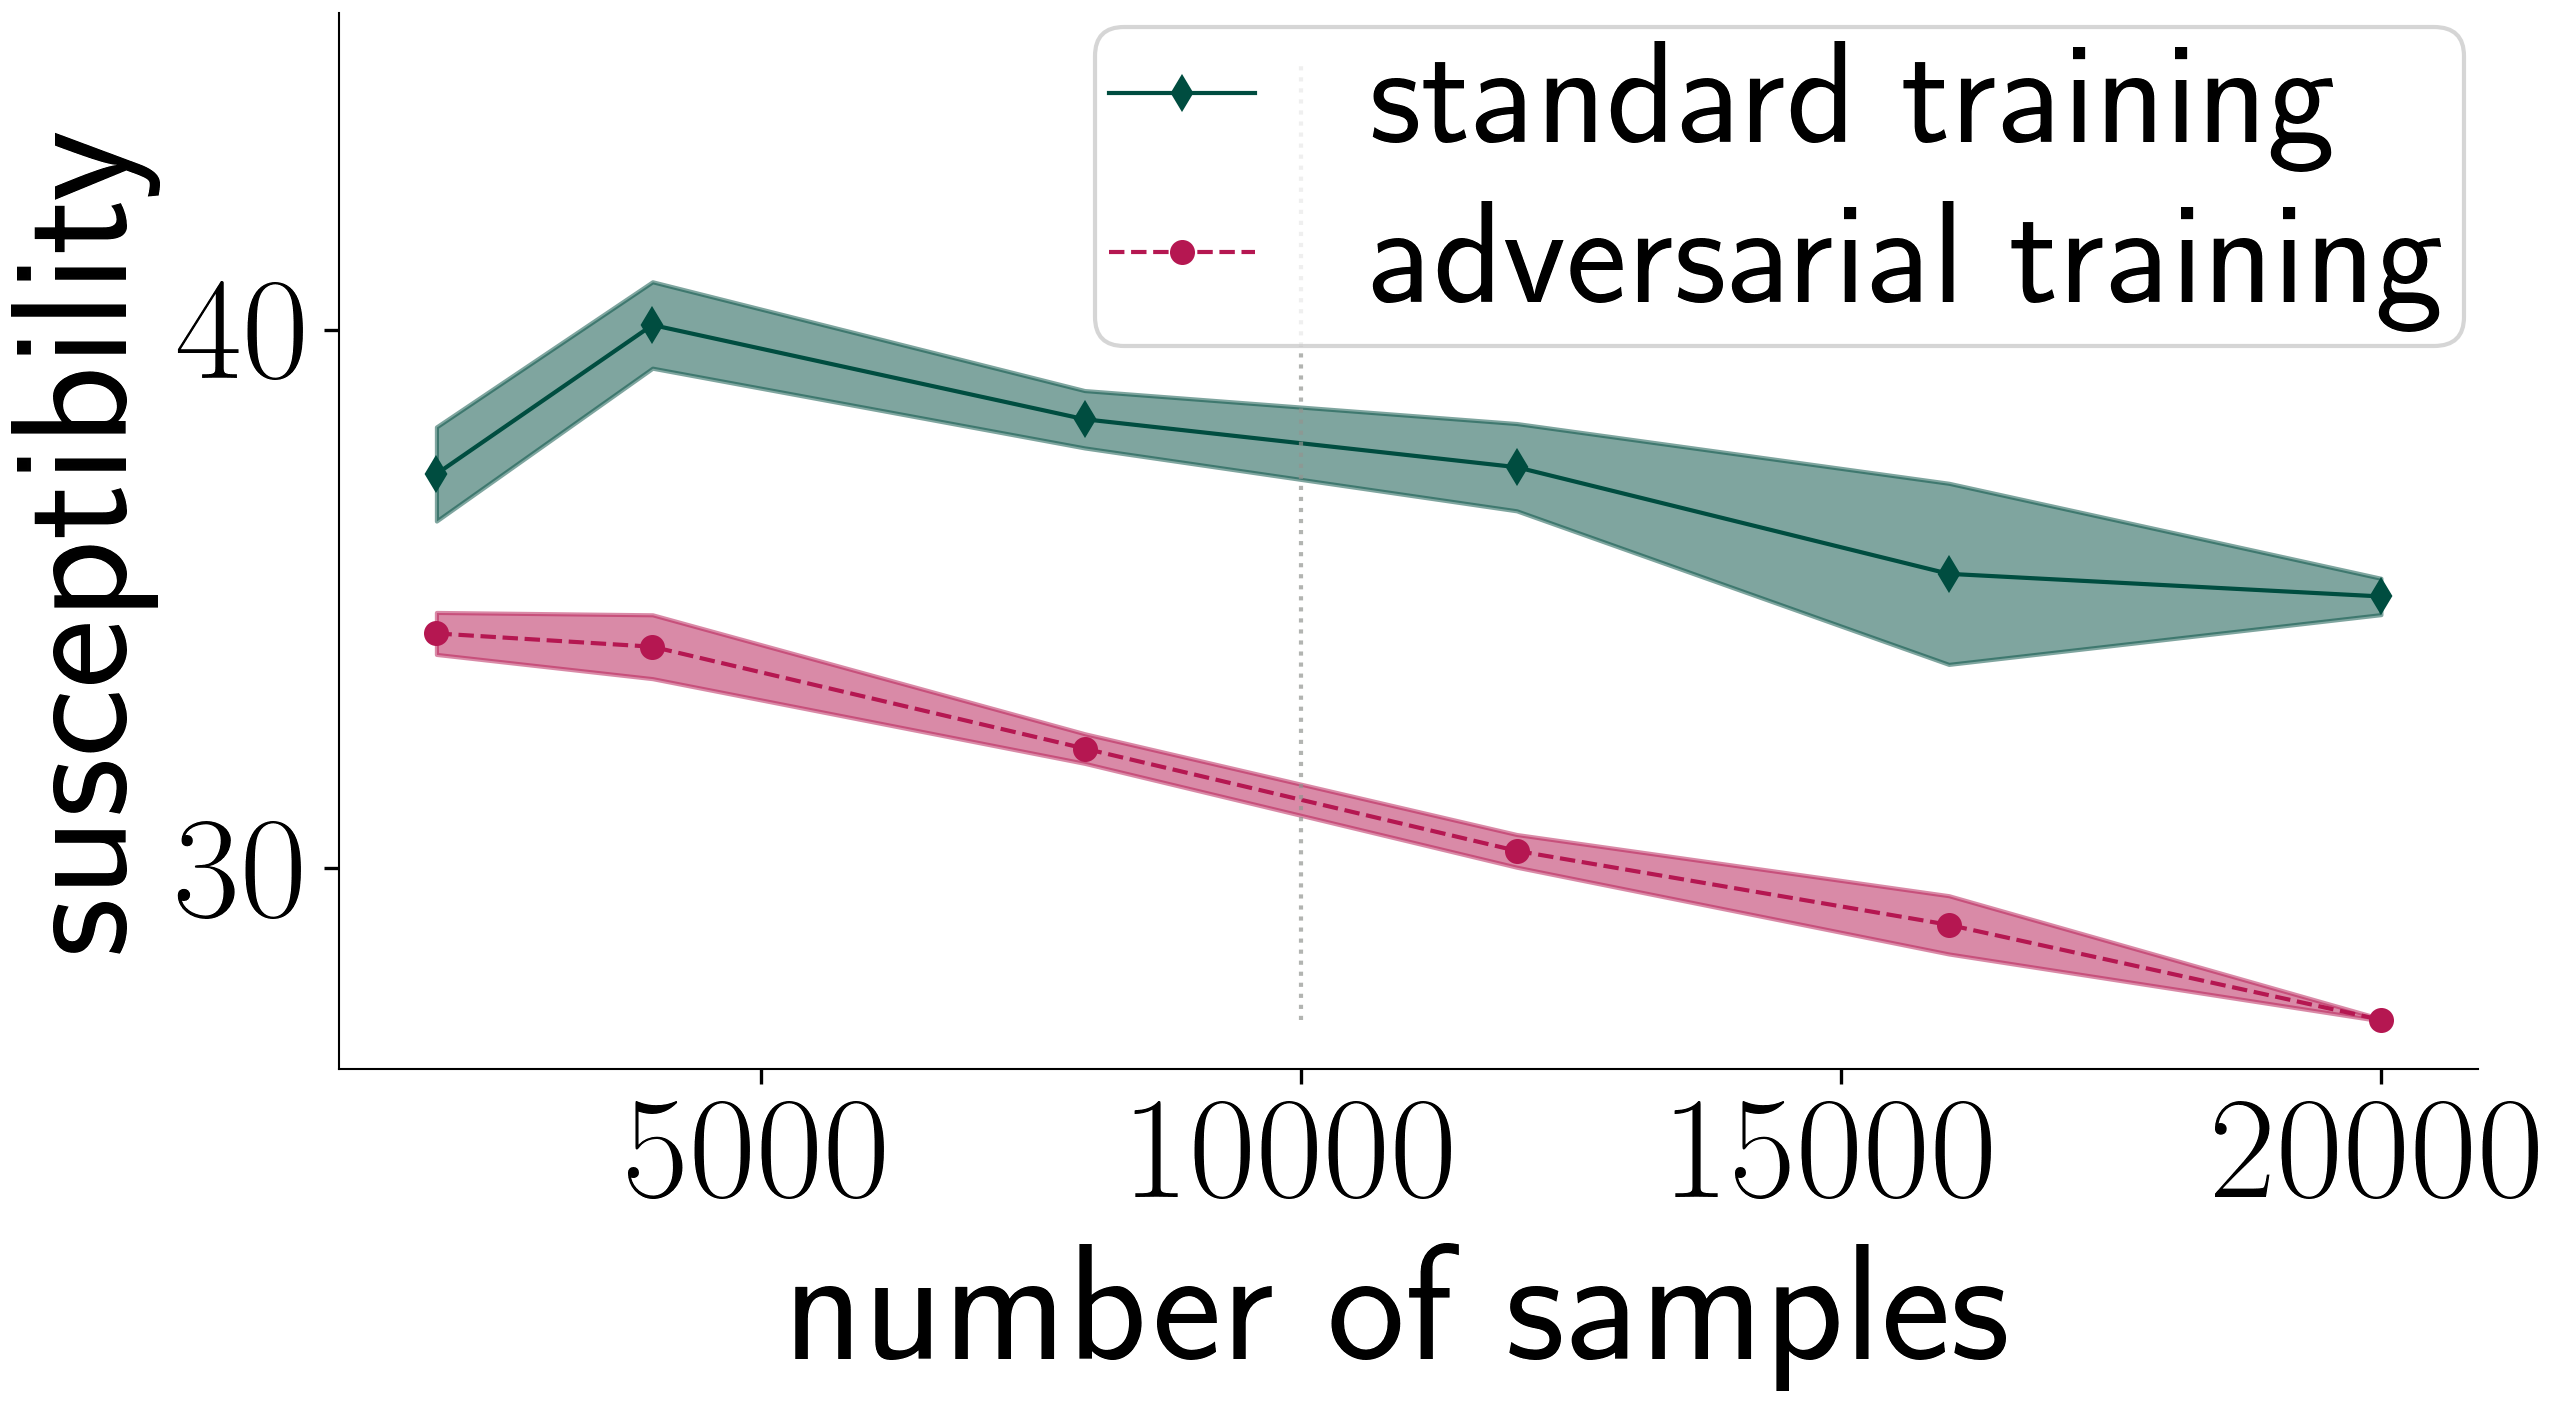
\includegraphics[width=0.99\linewidth]{plotsAistats/cifar10_sus_numobs.png}
  \caption{Susceptibility}
  \label{fig:Robustness_n}
\end{subfigure}

\caption{We plot the standard error, robust error and susceptibility of the subsampled datasets of 
CIFAR10 after adversarial and standard training. For small sample size, adversarial 
training has higher robust error then standard training. We see that the increase in standard error in comparison to the drop in susceptibility of standard versus robust training, switches between the low and high sample size regimes.}
\label{fig:num_obs_CIFAR}
\end{figure*}

\paragraph{Multiple networks on CIFAR10}
We run adversarial training for multiple network architectures on subsampled CIFAR10 ($n=500$) with mask perturbations of size $2 \times 2$ and an attack strength of $K=4$.  We plot the results in Table \ref{CIFAR10_diffArchitectures}. For all the different architectures, we notice a similar increase in robust error when trained with adversarial training instead of standard training.

\begin{table}[!ht]
\centering
\caption{We subsample CIFAR10 to a dataset of sample size $500$ and perform both standard training (ST) and adversarial training (AT) using different networks. We evaluate the resulting susceptibility score and the robust and standard error. }
\begin{tabular}{ |p{2cm}||p{2cm}||p{1cm}||p{1cm}|p{2cm}|p{2cm}|p{2cm}|}
 \hline
 \multicolumn{7}{|c|}{Adversarial training on CIFAR10} \\
 \hline
Architecture & learning rate & weight decay & Train type & standard error & robust error & Susceptibility\\
 \hline
 ResNet34 &   $ 0.02$  & $0.025$ &   ST  & 44 & 64 & 50 \\
 ResNet34 &   $0.015$  & $10^{-4}$ &   AT & 52 & 66 & 40\\
 ResNet50 &  $0.015$  & $0.03$  &   ST &  45 & 62 & 47\\
 ResNet50 &  $0.015$  &  $10^{-4}$ &   AT &  53 & 68 & 45\\
VGG11bn &  $0.03$ & $0.01$ & ST & 40 & 55 & 43\\
VGG11bn &   $0.015$  & $10^{-4}$ & AT & 48 &63 & 34\\
VGG16bn &  $0.02$ & $0.01$ & ST & 41 & 60 & 48\\
VGG16bn &   $0.015$  & $10^{-4}$ & AT & 50 & 65  & 42\\
 \hline
\end{tabular}
\label{CIFAR10_diffArchitectures}
\end{table}

%\fy{don't really see the relevance of the detail in this discussion
 % here} To give further insights on how the robustness and standard
%metrics behave as a function of sample size, we run adversarial and
%standard training on datasets of sizes $4 \cdot 10^{3}$ to $2 \cdot
%10^{4}$ and compare robustness, standard and robust accuracy. We plot
%the results in Figure \ref{fig:num_obs_CIFAR}.  Right of the gray
%line, corresponding to a dataset size of approximately $10^{4}$
%samples and larger, we recognise the known regime where adversarial
%training causes a drop in standard accuracy, but gains some robust
%accuracy. However, at the left side of the gray lines in Figure
%\ref{fig:num_obs_CIFAR} we note that adversarial training increases
%robustness, but standard accuracy drops by a larger margin causing
%robust accuracy to decrease. Full experimental details are provided in
%Section \ref{sec:app_cifar10}. Similar experiments for SVHN can be
%found in Appendix \ref{sec:app_SVHN}.